\section{ANN-Based Link-Risk Prediction}
The controller predicts the next-slot link margin before scheduling. For every feasible swarm-cluster pair, the feature vector $\vect{z}_{s,k,t}$ includes swarm and cluster identifiers, distance, elevation angle, relative speed, weather state, frequency, bandwidth, transmit power, previous link margin, previous outage flag, cache-hit flag, residual energy, current load, and normalized time. The ANN is an MLP with three hidden layers of 64 ReLU neurons. The output is the predicted next-slot link margin:
\begin{equation}
\hat{m}_{s,k,t+1}=f_{\theta}(\vect{z}_{s,k,t}).
\label{eq:ann_margin}
\end{equation}

The margin prediction is converted into outage risk using weather-wise residual calibration:
\begin{equation}
\hat{p}^{\mathrm{out}}_{s,k,t}=\sigma\left(\frac{m_{\mathrm{th}}-\hat{m}_{s,k,t+1}}{\sigma_w}\right),
\label{eq:outage_risk}
\end{equation}
where $m_{\mathrm{th}}$ is the outage margin threshold, $\sigma_w$ is the calibrated residual scale for weather state $w$, and $\sigma(\cdot)$ is the sigmoid function. This risk value is used in both service estimation and scheduling.

\begin{algorithm}[!t]
\caption{ANN-Based Link-Risk Prediction}
\label{alg:link_prediction}
\begin{algorithmic}[1]
\REQUIRE Feature vector $\vect{z}_{s,k,t}$, trained ANN $f_\theta$, weather state $w$, threshold $m_{\mathrm{th}}$, calibration scale $\sigma_w$
\ENSURE Predicted margin $\hat{m}_{s,k,t+1}$ and outage risk $\hat{p}^{\mathrm{out}}_{s,k,t}$
\STATE Collect distance, elevation angle, relative speed, weather, bandwidth, transmit power, previous margin, previous outage, cache flag, energy, load, and time features.
\STATE Normalize features using the predictor preprocessing rule.
\STATE Compute $\hat{m}_{s,k,t+1}=f_\theta(\vect{z}_{s,k,t})$.
\STATE Select weather-wise residual scale $\sigma_w$.
\STATE Compute $\hat{p}^{\mathrm{out}}_{s,k,t}=\sigma((m_{\mathrm{th}}-\hat{m}_{s,k,t+1})/\sigma_w)$.
\RETURN $\hat{m}_{s,k,t+1}$, $\hat{p}^{\mathrm{out}}_{s,k,t}$.
\end{algorithmic}
\end{algorithm}


The final paper-lock predictor results are shown in Tables~\ref{tab:predictor_metrics} and~\ref{tab:predictor_weather}. The overall RMSE is 4.592 dB and the Pearson correlation is 0.810. Weather-wise errors are not identical. The rain-hot state has the largest RMSE in the paper-lock predictor table, which matches the motivation that harsh weather causes wider residuals.

\begin{table}[!t]
\centering
\caption{Overall ANN link-margin predictor metrics on the paper-lock predictor evaluation set.}
\label{tab:predictor_metrics}
\scriptsize
\begin{tabular}{lccccc}
\toprule
MSE & RMSE & MAE & $R^2$ & Pearson $R$ & Time/sample (ms) \\
\midrule
21.090 & 4.592 & 3.865 & 0.554 & 0.810 & 0.0042 \\
\bottomrule
\end{tabular}
\end{table}

\begin{table}[!t]
\centering
\caption{Weather-wise link predictor error and calibrated residual scale.}
\label{tab:predictor_weather}
\scriptsize
\begin{tabular}{lcccccc}
\toprule
Weather & MSE & RMSE & MAE & $R^2$ & Samples & $\sigma_w$ (dB) \\
\midrule
clear & 20.194 & 4.494 & 3.910 & 0.510 & 1332 & 4.711 \\
rain\_hot & 24.200 & 4.919 & 3.900 & 0.512 & 346 & 4.310 \\
rainy & 21.232 & 4.608 & 3.777 & 0.522 & 822 & 4.108 \\
\bottomrule
\end{tabular}
\end{table}


Fig.~\ref{fig:predictor_scatter} shows the predicted and true link margins, and Fig.~\ref{fig:predictor_residual} shows residuals by weather. These figures are used as predictor diagnostics and not as proof that the link model is complete.

\begin{figure}[!t]
\centering
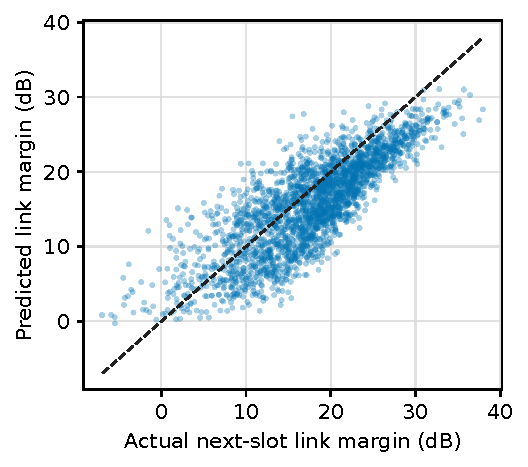
\includegraphics[width=\columnwidth]{figs/predictor_scatter_paperlock.pdf}
\caption{ANN link-margin prediction scatter on the paper-lock predictor evaluation set. The plot compares predicted and actual margins. The spread shows that prediction is useful but not exact.}
\label{fig:predictor_scatter}
\end{figure}

\begin{figure}[!t]
\centering
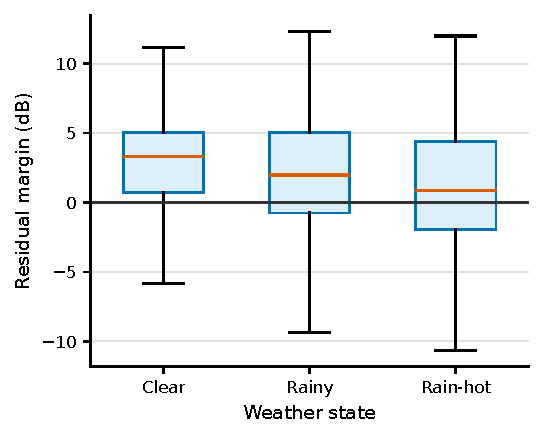
\includegraphics[width=\columnwidth]{figs/predictor_residual_by_weather_paperlock.pdf}
\caption{Prediction residuals by weather state. The rain-hot condition has wider error spread than easier weather states, so outage risk calibration is needed.}
\label{fig:predictor_residual}
\end{figure}
